\section{实验结果及分析}
% \textcolor{red}{需要仿真图一张,控制台打印输出图一张,要求仿真图中包含pc、instr、rs、rt、rd、result信号,仿真图应在控制台打印输出Simulation succeeded时截图。控制台打印输出图为此时截图。}
\subsection{仿真图}
\begin{figure}[H]
    \centering
    \caption{仿真图}
    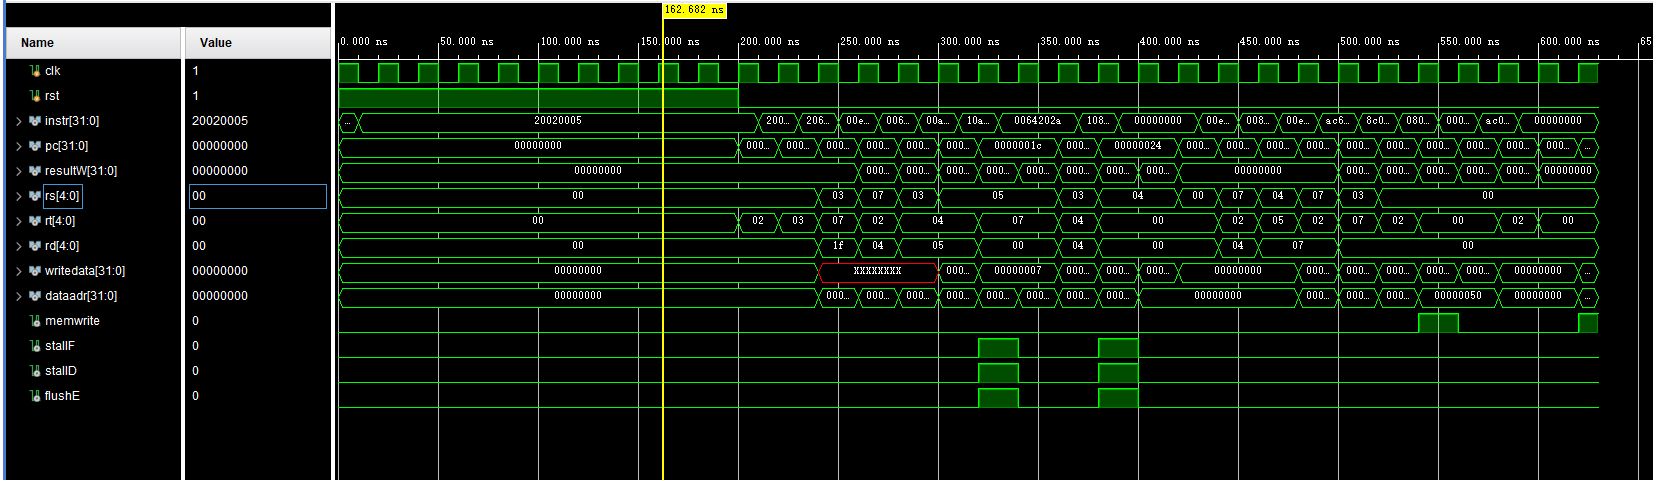
\includegraphics[width=1\textwidth]{figure/仿真.png}
    \label{fig:sim}
\end{figure}
\subsection{控制台}
\begin{figure}[H]
    \centering
    \caption{控制台输出}
    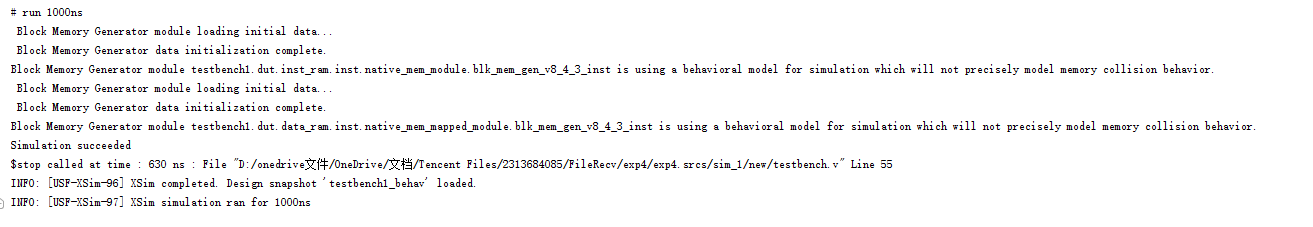
\includegraphics[width=1\textwidth]{figure/控制台.png}
    \label{fig:console}
\end{figure}
\subsection{仿真结束}
\begin{figure}[H]
    \centering
    \caption{仿真结束}
    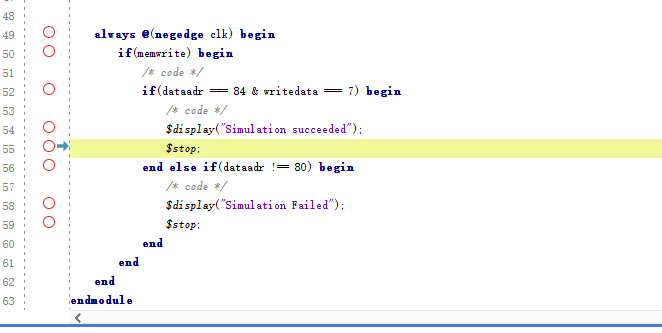
\includegraphics[width=0.8\textwidth]{figure/仿真结束.png}
    \label{fig:sim_stop}
\end{figure}